\documentclass[10pt]{standalone}
\usepackage{commands}

\begin{document}
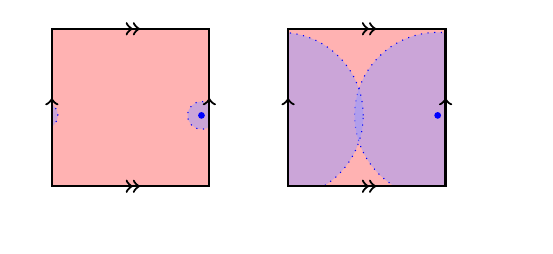
\begin{tikzpicture}[scale=1]
    \draw[black, thick, fill = white!70!red] (3, 0) -- (5, 0) -- (5, 2) -- (3, 2) -- cycle;
    \draw[dotted, blue, fill=white!60!blue, fill opacity=0.5] (4.9, 0.9) circle (30pt);
    \draw[dotted, blue, fill=white!60!blue, fill opacity=0.5] (2.9, 0.9) circle (30pt);

    \draw[draw=white, fill=white] (2.3, -0.3) -- (2.3, 2) -- (2.98, 2) -- (2.98, -0.3) -- cycle;
    \draw[draw=white, fill=white] (5.02, -0.3) -- (5.02, 2) -- (6, 2) -- (6, -0.3) -- cycle;
    \draw[draw=white, fill=white] (2.98, -0.02) -- (5.02, -0.02) -- (5.02, -0.5) -- (2.98, -0.5) -- cycle;
    \draw[fill=blue, draw=blue] (4.9, 0.9) circle (1pt);
    \draw[thick] (3, 0) -- (3, 2) -- (5, 2) -- (5, 0) -- cycle;
    \draw[->, thick] (3, 0) -- (3, 1.12);
    \draw[->, thick] (5, 0) -- (5, 1.12);
    \draw[->>, thick] (3, 0) -- (4.12, 0);
    \draw[->>, thick] (3, 2) -- (4.12, 2);

    \draw[black, thick, fill = white!70!red] (0, 0) -- (2, 0) -- (2, 2) -- (0, 2) -- cycle;
    \draw[dotted, blue, fill=white!60!blue, fill opacity=0.5] (1.9, 0.9) circle (5pt);
    \draw[dotted, blue, fill=white!60!blue, fill opacity=0.5] (-0.1, 0.9) circle (5pt);
    \draw[draw=white, fill=white] (-0.3, 0) -- (-0.3, 2) -- (-0.02, 2) -- (-0.02, 0) -- cycle;
    \draw[draw=white, fill=white] (2.02, 0) -- (2.02, 2) -- (2.3, 2) -- (2.3, 0) -- cycle;
    \draw[fill=blue, draw=blue] (1.9, 0.9) circle (1pt);
    \draw[->, thick] (0, 0) -- (0, 1.12);
    \draw[->, thick] (2, 0) -- (2, 1.12);
    \draw[->>, thick] (0, 0) -- (1.12, 0);
    \draw[->>, thick] (0, 2) -- (1.12, 2);

\end{tikzpicture}
\end{document}